\section{Задание 1. Замена базиса.}

\textbf{Условие.}

В параллелограмме $ABCD$ точка $E$ лежит на стороне $BC$, а точка $F$ – на стороне $AB$, причем $\displaystyle \frac{|BE|}{|BC|} = \frac{1}{4}$, $\displaystyle \frac{|BF|}{|AF|} = \frac{2}{5}$.
Найти координаты точки плоскости в системе координат $C$, $\overrightarrow{CE}$ , $\overrightarrow{CD}$,
если известны ее координаты $x^\prime$, $y^\prime$ в системе координат $E$, $\overrightarrow{EF}$ , $\overrightarrow{ED}$.
\vspace{10mm}

\textbf{Решение.}

Построим график. \\
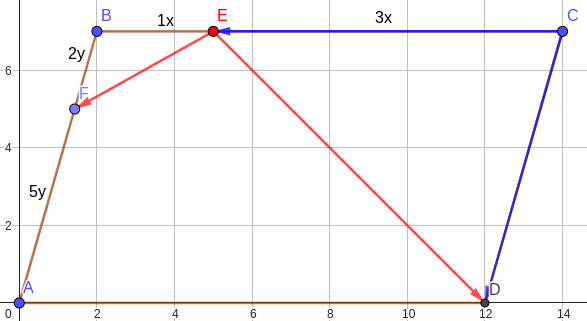
\includegraphics[width=0.9\linewidth]{images/1_grafik.png}

Пусть нам дана точка $M(x^\prime,~y^\prime)$ в СК $E,~\overrightarrow{EF},~\overrightarrow{ED}$ \\
Найдём координаты точки $C$ в этой СК:  \\

	$\overrightarrow{EC} = \overrightarrow{ED} + \overrightarrow{DC} $ \\
	$\overrightarrow{EF} = \overrightarrow{EB} + \overrightarrow{BF} = \frac{1}{4} \overrightarrow{CB} + \frac{2}{7} \overrightarrow{BA} = \frac{1}{4} \overrightarrow{CB} + \frac{2}{7} \overrightarrow{CD} \Longrightarrow \frac{-2}{7} \overrightarrow{CD} = \frac{1}{4} \overrightarrow{CB} - \overrightarrow{EF} $ \\ 
	$\overrightarrow{DC} = \frac{7}{8} \overrightarrow{CB} - \frac{7}{2} \overrightarrow{EF} $ \\ 
	$\overrightarrow{EC} = \overrightarrow{ED} + \frac{7}{8} \overrightarrow{CB} - \frac{7}{2} \overrightarrow{EF} $ \\
	$\overrightarrow{CB} = -\frac{4}{3} \overrightarrow{EC} $ \\ 
	$\overrightarrow{EC} = \overrightarrow{ED} - \frac{7}{6} \overrightarrow{EC} - \frac{7}{2} \overrightarrow{EF} $ \\
	$\frac{13}{6} \overrightarrow{EC} = \overrightarrow{ED} - \frac{7}{2} \overrightarrow{EF} $ \\
	$\overrightarrow{EC} = \frac{6}{13} \overrightarrow{ED} - \frac{21}{13} \overrightarrow{EF} $ \\

Итак, координаты точки $C:~(\frac{21}{13}, -\frac{6}{13})$ \\

Совершим перенос на вектор $\overrightarrow{EC}(-\frac{21}{13}, \frac{6}{13})$: найдём координаты точки $M(x^{\prime\prime},~y^{\prime\prime})$ в СК $C,~\overrightarrow{EF},~\overrightarrow{ED}$ \\
	$
		\begin{cases}
			x^{\prime\prime} = x^\prime + \frac{21}{13} \\ 
			y^{\prime\prime} = y^\prime - \frac{6}{13} \\
		\end{cases}
	$

Представим вектора $\overrightarrow{EF},~\overrightarrow{ED}$ как сумму векторов $\overrightarrow{CE},~\overrightarrow{CD}$ \\
	
	$\overrightarrow{EF} = \frac{1}{4} \overrightarrow{CB} + \frac{2}{7} \overrightarrow{CD} $ \\
	$\overrightarrow{CB} = \frac{4}{3} \overrightarrow{CE} \Longrightarrow \overrightarrow{EF} = \frac{1}{3} \overrightarrow{CE} + \frac{2}{7} \overrightarrow{CD}$ \\
	$\overrightarrow{ED} = \overrightarrow{EC} + \overrightarrow{CD} = -\overrightarrow{CE} + \overrightarrow{CD} $ \\
\\
Координаты $M$ в СК $C,~\overrightarrow{EF},~\overrightarrow{ED}$ - $(x^{\prime\prime},~y^{\prime\prime})$ $\Longrightarrow$ $\overrightarrow{CM} = x^{\prime\prime} \overrightarrow{EF} + y^{\prime\prime} \overrightarrow{ED}$ \\
$\overrightarrow{CM} = x^{\prime\prime} (\frac{1}{3} \overrightarrow{CE} + \frac{2}{7} \overrightarrow{CD}) + y^{\prime\prime} (-\overrightarrow{CE} + \overrightarrow{CD})$ \\
$\overrightarrow{CM} = (\frac{1}{3}x^{\prime\prime}  - y^{\prime\prime}) \overrightarrow{CE} + (\frac{2}{7}x^{\prime\prime} + y^{\prime\prime}) \overrightarrow{CD} $ \\

Найдём координаты точки $M(x,~y)$ в СК $C,~\overrightarrow{CE},~\overrightarrow{CD}$ \\
	$
		\begin{cases}
			x = \frac{1}{3}x^{\prime\prime} - y^{\prime\prime} \\ 
			y = \frac{2}{7}x^{\prime\prime} + y^{\prime\prime} \\
		\end{cases}
	$ \\
Подставим в систему уравнения для $x^{\prime\prime},~y^{\prime\prime}$, полученные при переносе. \\
	$
		\begin{cases}
			x = \frac{1}{3}(x^\prime + \frac{21}{13}) - (y^\prime - \frac{6}{13}) \\ 
			y = \frac{2}{7}(x^\prime + \frac{21}{13}) + (y^\prime - \frac{6}{13}) \\
		\end{cases}
		\\
		\begin{cases}
			x = \frac{1}{3} x^\prime - y^\prime + 1 \\ 
			y = \frac{2}{7} x^\prime + y^\prime \\
		\end{cases}
	$ \\

Проверим построением. \\
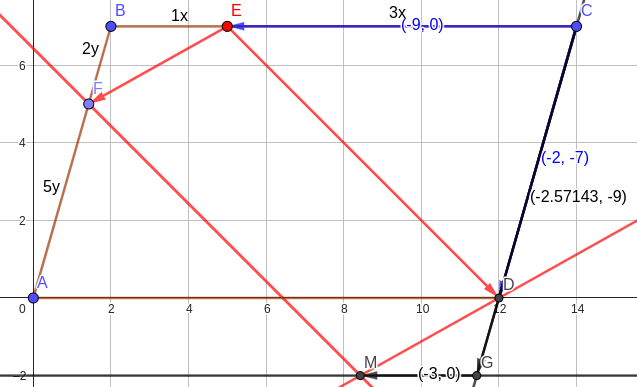
\includegraphics[width=0.9\linewidth]{images/1_proverka.png} \\
Возьмём точку $M$ с координатами $(1, 1)$ в СК $E,~\overrightarrow{ED},~\overrightarrow{ED}$ \\
По построению координаты точки в СК $C,~\overrightarrow{CE},~\overrightarrow{GM}$ равны $(\frac{|GM|}{|CE|}, \frac{|CD|}{|CG|})$ \\
Найдём исходя из СК, изображённой на рисунке ($A:~(0, 0),~B:~(2, 7)$): $M:~(\frac{3}{9}, \frac{9}{7})$ \\
Можно сократить до $M:~(\frac{1}{3},~\frac{9}{7})$ \\
По уравнениям координаты должны быть: $x = \frac{1}{3} - 1 + 1 = \frac{1}{3},~y = \frac{2}{7} + 1 = \frac{9}{7}$ \\

\textit{Ответ}: $M(\frac{1}{3} x^\prime - y^\prime + 1,~\frac{2}{7} x^\prime + y^\prime )$
\clearpage
